%!TEX root = /Users/markelikalderon/Documents/Git/formwithoutmatter/aristotle.tex
\chapter{Light and Dark} % (fold)
\label{cha:light_and_dark}

\section{Chromatic Harmony} % (fold)
\label{sec:chromatic_harmony}
The presence of the fiery substance\index{fiery substance} illuminates the potentially transparent\index{transparency} me\-di\-um\index{medium}. White\index{white} (\emph{leukon}\index{leukon@\emph{leukon}}) corresponds to the presence of this determinant of what is actually transparent. Conversely, black\index{black} (\emph{melaton}\index{melaton@\emph{melaton}}) corresponds to its absence\index{absence}. The absence of the fiery substance darkens\index{dark} the potentially transparent medium. White and black are thus associated with a fundamental condition on the visibility of remote external particulars.\index{color!generation of the hues} No doubt in part because of this Aristotle attempts to explain the other hues\index{hue} in terms of the ratio of white and black. He considers three such accounts, in terms of (1) juxtaposition\index{juxtaposition model}, (2) overlap\index{overlap model}, and (3) mixture\index{mixture model}, advocating the third. On all three accounts chromatic hues are determined by white\index{white} and black\index{black} in various ratios, the accounts differing only in how these ratios are implemented. 

The fundamental idea common to all three accounts can seem surprising. How can the ratio\index{ratio} of white and black result in something appearing red\index{red}? Would it not instead appear gray\index{gray}? Thus \citet[210]{Hett:1936fk}\index{Hett, W.S.} writes that Aristotle's ``doctrine could hardly have survived a few experiments with pigments''\index{pigment}. If Aristotle's account were disconfirmable by elementary experiments with pigment mixtures, then why did he not investigate the matter? Was it merely to avoid Plato's\index{Plato} charge of impiety\index{impiety}?
\begin{quote}
    There will be no difficulty in seeing how and by what mixtures the colors derived from these are made according to the rules of probability. He, however, who should attempt to verify all this by experiment would forget the difference between human and divine nature. For God only has the knowledge and also the power which are able to combine many things into one and again resolve the one into many. But no man either is or ever will be able to accomplish either the one or the other operation. (Plato, \emph{Timaeus} 68\( ^{d} \); Jowett in \citealt[1192]{Hamilton:1989fk})\index{Timaeus@\emph{Timaeus}}
\end{quote}
The impiety of mixture will be echoed by Plutarch\index{Plutarch} in the first century \textsc{ad}:
\begin{quote}
	Mixing\index{mixture} produces conflict, conflict produces change\index{change}, and putrefaction is a kind of change. This is why painters call a blending of colours a `deflowering' and Homer calls dyeing `tainting,' and common usage regards the unmixed and pure as virgin and undefiled. (Plutarch, \emph{Moralia}, Table-Talk (\emph{Quaestiones convivales}) \textsc{viii} 5 725\( ^{c-d} \); Minar in \citealt[155--157]{Milnar:1961aa})\index{Moralia, Quaestiones convivales@\emph{Moralia, Quaestiones convivales}}\index{Plutarch}
\end{quote}

Aristotle's account of the generation of the hues\index{color!generation of the hues} may be surprising, but it would be wrong to prematurely dismiss it. The first thing to observe is that \emph{leukon}\index{leukon@\emph{leukon}} and \emph{melaton}\index{melaton@\emph{melaton}} are better understood as light\index{light} and dark\index{dark}, rather than white\index{white} and black\index{black}. There is a general tendency in Greek color vocabulary to classify colors in terms of relative brightness\index{bright} rather than hue\index{hue} \citep[see][]{Gladstone:1858fk,Platnauer:1921bh,Osbourne:1968vn,Lloyd:2007fk}\index{Gladstone, W.E.}\index{Platnauer, Maurice}\index{Osbourne, H.}\index{Lloyd, G.E.R.}. Traces of such a usage exist in English. Thus we speak of white wine and white people, though neither are white in hue. Similarly neither black people nor black grapes are black in hue. This usage in English, however, does not seem to be perfectly general but is rather lexically determined. It is not the case that ``white'' can be interpreted in terms of relative brightness instead of hue when applied to just any noun. The availability of such an interpretation seems to be limited to the adjective's application to certain nouns. The more general usage in Greek is philosophically significant, for it transforms Aristotle's claim. Aristotle is not claiming that the hues are determined by the ratio\index{ratio} of white and black, but that they are determined by the ratio of light\index{light} and dark\index{dark}. Experiments with pigment mixtures\index{pigment}\index{mixture} are irrelevant to the truth of this latter claim. Thus, Aristotle need not have risked Plato's\index{Plato} charge of impiety\index{impiety} as Hett\index{Hett, W.S.} recommends. Not only is the thought that the hues\index{hue} are determined by the ratio\index{ratio} of light\index{light} and dark\index{dark} not disconfirmable by impious experimentation, it is independently plausible. (Indeed, as I will argue in chapter~\ref{sec:assessment}, it is an ancient prefiguration of modern reflectance theories, see \citealt{Hilbert:1987jq}.)\index{color!reflectance theory}\index{Hilbert, David R.}

Two further considerations are relevant. First, there are a range of observable phenomena that support Aristotle's fundamental claim that a ratio\index{ratio} of white\index{white} and black\index{black} or light\index{light} and dark\index{dark} can give rise to chromatic appearances. Importantly, Aristotle himself provides an example. Second, Aristotle's account has ancient precedent. Thus when Theophrastus\index{Theophrastus} discusses Democritus's\index{Democritus} view that there are four primary colors\index{color!primary} (understood as simple colors in terms of which all other colors are to be explained), he contrasts it with the then dominant view that white and black are the two primary colors:
\begin{quote}
    But first of all, his increase of the number of primaries presents a difficulty; for the other investigators propose white and black as the only simple colours. (Theophrastus, \emph{De Sensibus} \textsc{lvix}; \citealt[137]{Stratton:1917vn})\index{De Sensibus@\emph{De Sensibus}}\index{Theophrastus}
\end{quote}
It is reasonable to suppose that Aristotle's account of the generation of the hues\index{color!generation of the hues} draws on this pre-Democritean tradition. Before discussing Aristotle's account of the generation of the hues, then, I will review some empirical support for its central idea, and will discuss the precedent for this doctrine in Parmenides\index{Parmenides} and Empedocles\index{Empedocles}.

% section chromatic_harmony (end)

\section{Empirical Support} % (fold)
\label{sec:empirical_support}
In 1894, an English toy maker, Charles Benham\index{Benham, Charles}, devised a top adorned with a black and white pattern (see Figure~\ref{fig:2}). Sold through Messrs. Newton and Co., an announcement of the ``Artificial Spectrum Top''\index{Artificial Spectrum Top|seealso{Benham disk}} was published in \emph{Nature}:
	\begin{quote}
		The top consists of a disc, one half of which is black, while the other half has twelve arcs of concentric circles drawn upon it. Each arc subtends an angle of forty-five degrees. In the first quadrant there are three such concentric arcs, in the next three more, and so on; the only difference being that the arcs are parts of circles of which the radii increase in arithmetical progression. Each quadrant thus contains a group of arcs differing in length from those of the other quadrants. The curious point is that when this disc is revolved, the impression of concentric circles of different colors is produced upon the retina. If the direction of rotation is reversed, the order of these tints is also reversed. \citep{Benham:1894kx}
	\end{quote}
Specifically, if rotated clockwise, the innermost arcs form reddish\index{reddish} rings, the next greenish\index{greenish} rings, the next light blue\index{blue} rings, and the outermost arcs form violet\index{violet} rings. If rotated counterclockwise, the pattern is reversed with the innermost arcs now forming violet rings and the outermost reddish rings. The apparent colors of Benham's spinning disk\index{Benham disk} are the ``subjective colors'' first described by \citep{Fechner:1838vn}\index{Fechner, F.T.} and, hence, are also sometimes described as ``Fechner-Benham colors''.

\begin{figure}[ht]
    \begin{center}
        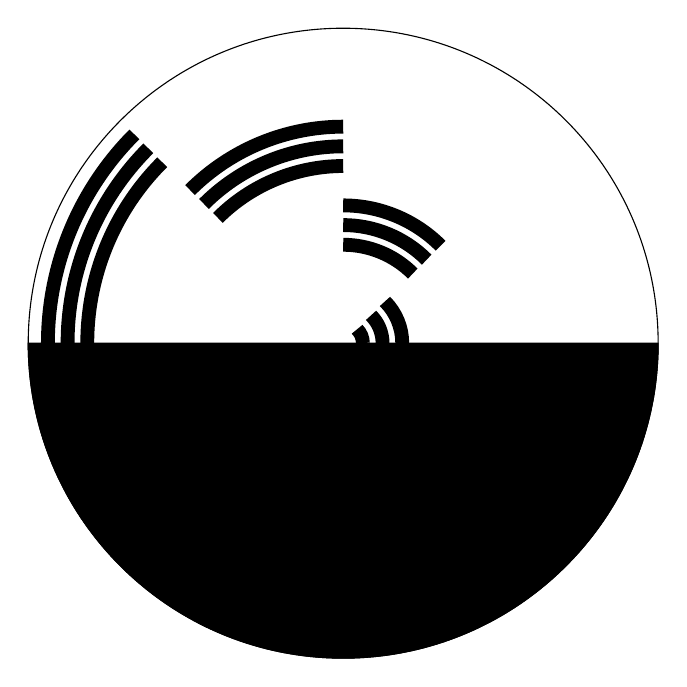
\begin{tikzpicture}
			\draw (0,0) circle (4cm);
			\filldraw[fill=black] (0,0) -- (4cm,0cm) arc (0:-180:4cm) --cycle;
			\draw[line width=5pt] (canvas polar cs:angle=0,radius=0.25cm) arc (0:45:0.25cm);
			\draw[line width=5pt] (canvas polar cs:angle=0,radius=0.50cm) arc (0:45:0.50cm);
			\draw[line width=5pt] (canvas polar cs:angle=0,radius=0.75cm) arc (0:45:0.75cm);
			\draw[line width=5pt] (canvas polar cs:angle=45,radius=1.25cm) arc (45:90:1.25cm);
			\draw[line width=5pt] (canvas polar cs:angle=45,radius=1.50cm) arc (45:90:1.50cm);
			\draw[line width=5pt] (canvas polar cs:angle=45,radius=1.75cm) arc (45:90:1.75cm);
            \draw[line width=5pt] (canvas polar cs:angle=90,radius=2.25cm) arc (90:135:2.25cm);
			\draw[line width=5pt] (canvas polar cs:angle=90,radius=2.50cm) arc (90:135:2.50cm);
			\draw[line width=5pt] (canvas polar cs:angle=90,radius=2.75cm) arc (90:135:2.75cm);
			\draw[line width=5pt] (canvas polar cs:angle=135,radius=3.25cm) arc (135:180:3.25cm);
			\draw[line width=5pt] (canvas polar cs:angle=135,radius=3.50cm) arc (135:180:3.50cm);
			\draw[line width=5pt] (canvas polar cs:angle=135,radius=3.75cm) arc (135:180:3.75cm);
		\end{tikzpicture}
    \end{center}
    \caption{The Benham Disk or ``Artificial Spectrum Top''}
    \label{fig:2}
\end{figure}

Consider a puzzling aspect of the subjective colors of the Benham disk\index{Benham disk}. Each of the spinning arcs reflect light with the same spectral content and with equal average luminance. In advance of observing the spinning disk, one might reasonably expect the spinning arcs to appear as gray rings of equal brightness. Why, then, do the rings appear reddish, greenish, light blue, and violet? The subjective colors of the Benham disk are not completely understood \citep[for a review of some of the color science see][]{Campenhausen:1995yq}\index{Campenhausen, Christoph von}\index{Schramme, J\"{u}rgen}. However, this much is clear: The innermost ring appearing reddish is the result of the visual system integrating temporal inhomogeneities presented by the spinning disk. Presentations of black and white stimuli altering at a particular temporal ratio elicits a chromatic response in normal human perceivers. 

This basic principle was used in a prototype of color television \citep[]{Butterfield:1968uq,Butterfield:1970kx}. Developed by James F. Butterfield\index{Butterfield, James F.} (who studied philosophy at the University of Chicago as an undergraduate), the broadcasting system consists of the Butterfield color encoder\index{Butterfield color encoder} that produces a monochromatic signal that when broadcast and displayed on a black-and-white monitor presents a chromatic appearance. The Butterfield encoder extracts a monochromatic signal from the colored scene by passing the light from the scene through cyan\index{cyan}, magenta\index{magenta}, and yellow\index{yellow} filters. The filters themselves are arranged in, what is in effect, a modified Benham disk\index{Benham disk}. The bottom half of the filter is opaque\index{opacity} with the colored filters fanned across the top half. The filters thus form a disk which is rotated. A colored object will appear black\index{black} when seen through a filter of a complementary color. This and the opaque half of the rotating disk produces a pulsed black-and-white signal that elicits a chromatic response in normal human perceivers. The system produced good skin tones but unmixed hues, especially red\index{red}, tended to flicker. The initial public demonstration was, by all accounts, startling:
\begin{quote}
    When electronic color was first publicly demonstrated in the Los Angeles area over KNXT, no prior announcement had been made at the request of a soft-drink manufacturer sponsoring the test. The beverage firm wanted its color commercials to be a complete surprise to viewers of black-and-white receivers. And, the telecasts were that, to say the very least. Within hours of the electronic-color broadcast, thousands of viewers began asking the same question, ``What happened? Did I really see color on my black-and-white receiver? Or am I having hallucinations?'' \citep[]{Griffin:1968fk}\index{Griffin, Laurence R.}
\end{quote}
The power to demand such attention did not go unnoticed. The final public demonstration was an Eva Per\'{o}n\index{Eva Per\'{o}n} political advertisement.

That the pulsed black-and-white signal produced by the Butterfield color encoder\index{Butterfield color encoder} gives rise to a chromatic appearance is once again the result of the visual system integrating temporal inhomogeneities. However, these temporal inhomogeneities are not the result of spatial movement of the object of perception, but rather due to the qualitative alterations over time of a stationary object. Each involves the presentation of white\index{white} and black\index{black} stimuli altering at a particular temporal ratio\index{ratio} eliciting a chromatic response in normal human perceivers. They differ in how that temporal ratio is implemented---by the motion of an object whose parts qualitatively differ or by the qualitative alteration over time of a stationary object. 

Stated so abstractly it is easy to see that there is a third possibility. If the temporal ratio that determines a given chromatic appearance can be implemented by the motion of a black and white object, the perceivers motion relative to a black\index{black} and white\index{white} object should do so as well. And indeed it can. Our eyes constantly scan the scene with involuntary saccades. Scanning a stationary black and white object can give rise to chromatic appearance \citep[72]{Hardin:1993kn}\index{Hardin, C.L.}. Thus Sorabji\index{Sorabji, Richard} claims that contemporary art provides an example:
\begin{quote}
    I also wrote about colour and vision in the 1970s. At Cornell, I had heard Edward Land, the inventor of the polaroid camera, lecture on his discovery that Newton’s\index{Newton, Issac} theory of colour is wrong. The eye responds not to absolute wavelengths of light, but to the more complicated property of reflectance, which involves the proportions among wavelengths in the available scene. Land\index{Land, Edwin} was able to cast on the screen at Cornell a slide showing all the colours of the garden, yet he was using wavelengths only from within the yellow waveband. I was intrigued that Goethe had also rejected Newton’s theory of colour, and praised Aristotle for his theory that the other hues are produced by combinations of the brightest and the darkest. This, according to Goethe, is the theory that any painter would accept. We had a reproduction in our hallway of a painting by Bridget Riley\index{Riley, Bridget} consisting of wavy black and white stripes. Some of our guests saw brilliant colours in it. Others merely felt giddy. I wrote to ask Bridget Riley what she thought of Goethe and Aristotle, but this time I did not get an answer. (\citealt[13]{Sorabji:2005fk}; see also \citealt[295]{Sorabji:2022qf}\index{Sorabji, Richard})
\end{quote}
The chromatic appearances that Riley's painting give rise to  are the result of the visual system integrating temporal inhomogeneities that result from the eye involuntarily moving across a stationary black and white object.

% (see Figure~\ref{fig:4})
% \begin{figure}[htbp]
%     \centering
%         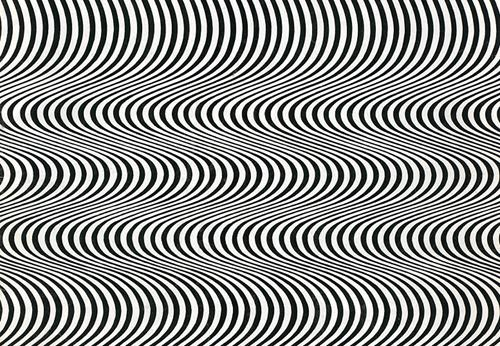
\includegraphics{graphics/current.jpg}
%     \caption{Bridget Riley, \emph{Current}}
%     \label{fig:4}
% \end{figure}

These examples involve artifacts and technology unavailable at Aristotle's time. And while they may make plausible for \emph{us} that ratios\index{ratio} of white\index{white} and black\index{black} can, sometimes at least, give rise to chromatic appearances, they could not have done so for Aristotle. What empirical observation available to Aristotle could have made vivid for him the possibility that chromatic appearances are the result of the ratio of light and dark in the perceived scene? An example discussed in the last chapter could give rise to the relevant experience. The sun\index{sun} is white, but it appears red\index{red} when seen through fog\index{fog} or a cloud of smoke\index{smoke} (\emph{De Sensu} \textsc{iii} 440\( ^{a} \)10--11)\index{De Sensu@\emph{De Sensu}}.  The white\index{white} sun\index{sun}, when superimposed by black\index{black} particles suspended in the intervening transparent medium, looks red\index{red}. The reduction of the sun's brilliance by the intervening particulate matter of the smoke results in the sun's crimson appearance. In his \emph{Theory of Colors}, Goethe\index{Goethe, Johan Wolfgang von} repeats and elaborates Aristotle's example:
\begin{quote}
	The highest degree of light\index{light}, such as that of the sun, of phosphorus\index{phosphorus} burning in oxygen, is dazzling and colourless; so the light of the fixed stars\index{stars} is for the most part colourless. This light, however, seen through a medium but very slightly thickened, appears to us yellow\index{yellow}. If the density of the medium be increased, or if its volume become greater, we shall see the light gradually assume a yellow-red\index{yellow-red} hue, which at last deepens to a ruby-colour. \citep[\textsc{i} 10 150]{Goethe:1810uq}
\end{quote}
\begin{quotation}
	\noindent The sun seen through a certain degree of vapour appears with a yellow\index{yellow} disk; the centre is often dazzling yellow when the edges are already red\index{red}. The orb seen through a thick yellow mist appears ruby-red (as was the case in 1794, even in the north); the same appearance is still more decided, owing to the state of the atmosphere, when the scirocco prevails in the southern climates: the clouds genrally surrounding the sun in the latter case are of the same colour, which is reflected again on all objects.
	
	The red hues of morning and evening are owing to the same cause. The sun\index{sun} is announced by a red\index{red} light, in shining through a greater mass of vapours. The higher he rises, the yellower and brighter the light becomes. \citep[\textsc{i} 10 154]{Goethe:1810uq}
\end{quotation}

What is presently important is a general feature of Aristotle's example: that a reduction of an object's brilliance can result in a chromatic appearance. That provides direct partial support for the claim that a proportion\index{proportion} of light\index{light} and dark\index{dark} can give rise to a chromatic appearance.

% section empirical_support (end)

\section{Parmenides} % (fold)
\label{sec:parmenides}
\index{Parmenides|(}
Theophrastus\index{Theophrastus} (\emph{De Sensibus} \textsc{lvix})\index{De Sensibus@\emph{De Sensibus}} alludes to a pre-Democritean tradition according to which white\index{white} and black\index{black} are the primary colors\index{color!primary}, the colors in terms of which all other colors are to be explained. While Theophrastus\index{Theophrastus} does not name any particular thinker belonging to this tradition, one may reasonably speculate. In his notorious study, among the five ``signs of the immaturity'' of the Homeric\index{Homer!color scheme} color scheme, Gladstone\index{Gladstone, W.E.} cites the following:  
\begin{quote}
    The vast predominance of the most crude and elemental forms of colour, black and white, over every other, and the decided tendency to treat other colours as simply intermediate modes between these two extremes. \citep[458]{Gladstone:1858fk}
\end{quote}
One can reasonably accept Gladstone's observation about the structure of the Ho\-meric color scheme, while bracketing any conclusions about relative deficiencies in the Greek's capacity to discriminate color or about their taste in color composition. It is ironic that just as archeological evidence for the widespread use of polychromacy\index{polychromacy} in classical sculpture emerges, Gladstone, in order to explain apparent anomalies in Greek color vocabulary, hypothesizes that the ancient Greeks were color blind. Amusingly, \citealt[162]{Platnauer:1921bh}\index{Platnauer, Maurice}, while tempted by Gladstone's\index{Gladstone, W.E.} diagnosis of color blindness among the ancient Greeks, accuses them instead of having bad taste in being insensitive to ``the qualitative differences of decomposed and partially absorbed light''. If we bracket such judgments, then arguably the pre-De\-mo\-cri\-tean tradition that Theophrastus alludes to has Homeric roots. Let us selectively examine this ancient tradition by attending to two key figures familiar to Aristotle, Parmenides and Empedocles (though the inclusion of the latter is controversial).

In the prologue to his poem, the goddess\index{unnamed goddess} promises to reveal to Parmenides two things, the Way of Truth\index{Parmenides!The Way of Truth} and the Way of Mortal Opinion\index{Parmenides!The Way of Mortal Opinion}. The doctrines of the latter she assures him are false; nevertheless, Parmenides must learn these too (\textsc{dk} 28\textsc{b}1.31). The Way of Mortal Opinion is an account of the world ``as it appears'' (\textsc{dk} 28\textsc{b}8.60; \citealt[155]{McKirahan:1994ve}), and the goddess\index{unnamed goddess} presents it to Parmenides ``so that no mortal opinion may ever overtake'' him (\textsc{dk} 28\textsc{b}8.61; \citealt[155]{McKirahan:1994ve}). The Way of Mortal Opinion\index{Parmenides!The Way of Mortal Opinion} is a cosmology in the Milesian tradition, though Parmenides is not expounding the views of any particular Milesian cosmologist \citep[on Parmenides and Milesian cosmology see][]{Kahn:1994qf}\index{Kahn, Charles H.}. Rather, he is presenting what is, by his lights, the best account that can be given along those lines. Traditional Milesian cosmologies tend to be monistic\index{monism}, but the Way of Mortal Opinion posits two fundamental and irreducible principles that stand in opposition, Fire\index{Parmenides!Fire} and Night\index{Parmenides!Night} or light\index{light} and dark\index{dark} (\textsc{dk} 28\textsc{b}8.53--61, 28\textsc{b}9). The thought seems to be this. Having shown, in the Way of Truth\index{Parmenides!The Way of Truth}, that monism\index{monism} is inconsistent with appearances, the Way of Mortal Opinion\index{Parmenides!The Way of Mortal Opinion} must posit a plurality of principles in opposition, if it is to accommodate the plurality and opposition encountered in the world as it appears in sensory experience. Or at least, this is the interpretation that Aristotle recommends:
\begin{quote}
    \ldots\ but being forced to follow the phenomena, and supposing that what is is one in formula but many according to perception, he now posits two causes and two principles, calling them hot and cold, \emph{i.e.} fire and earth. (Aristotle, \emph{Metaphysica} \textsc{a} 986\( ^{b} \)31; Ross in \citealt[12]{Barnes:1984kx})\index{Metaphysica@\emph{Metaphysica}}
\end{quote}

The two principles, Fire\index{Parmenides!Fire} and Night\index{Parmenides!Night}, of the Way of Mortal Opinion\index{Parmenides!The Way of Mortal Opinion}, have attributes called ``signs''\index{Parmenides!signs}:
\begin{verse}
    For they made up their minds to name two forms,\\ 
    Of which it is not right to name one---in this they have gone astray---\\
    And they distinguished things opposite in body, and established signs\\
    Apart from one another---for one, the aetherial fire\index{fire} of flame,\\
    Mild, very light, the same as itself in every direction,\\
    But not the same as the other; but that other one, in itself\\
    Is opposite---dark\index{dark} night\index{night}, a dense\index{dense} and heavy\index{heavy} body.\\
    I declare to you all the ordering as it appears,\\
    So that no mortal opinion may ever overtake you.
\end{verse}
\begin{verse}
    But since all things have been named light\index{light} and night\index{night}\\
    And the things which accord with their powers have been assigned to these things and those,\\
    All is full of light and obscuring night together,\\
    of both equally, since neither has no share.\\
    (Parmenides, \textsc{dk} 28\textsc{b}8.53--9.4; \citealt[155]{McKirahan:1994ve})
\end{verse}
Like Fire\index{Parmenides!Fire} and Night\index{Parmenides!Night} themselves, the attributes of these principles stand in opposition\index{Parmenides!signs}. Fire\index{Parmenides!Fire} is bright\index{bright}, Night\index{Parmenides!Night} is dark\index{dark}; Fire is rare\index{rare}, Night is dense\index{dense}, and so on. These attributes are sensible qualities arrayed in opposing contraries\index{contraries}\index{opposites}. Due to Parmenides's use of ambiguity---the signs of Fire and Night have multiple senses---\citet[244--245]{Mourelatos:2008ve}\index{Mourelatos, Alexander P.D.} argues that the system of sensible contraries is complex and one many. In contrast, the attributes of the one being of the Way of Truth\index{Parmenides!The Way of Truth} are not sensible (\emph{aistheton}) qualities\index{sensible qualities} arrayed in a system of contraries but intelligible (\emph{noeton}) properties (such as limit\index{limit} or unity).  Fire\index{Parmenides!Fire} and Night\index{Parmenides!Night} may have further attributes not listed here; much of the Way of Mortal Opinion\index{Parmenides!The Way of Mortal Opinion} is missing. A sense of its scope and ambition, however, is provided by Plutarch\index{Plutarch}:
\begin{quote}
    But Parmenides \ldots\ has actually made a cosmic order, and by blending as elements the light and the dark produces out of them and by their operation the whole world of sense. Thus he has much to say about earth\index{Earth}, heaven\index{heaven}, sun\index{sun}, moon\index{moon}, and stars\index{stars}, and has recounted the genesis of man; and for an ancient natural philosopher---who has put together a book of his own, and is not pulling apart the book of another---he has left nothing of real importance unsaid. (Plutarch, \emph{Adversus Colotem} 1114 b--c; \citealt[231]{Einarson:1967zr})\index{Adversus Colotem@\emph{Adversus Colotem}}
\end{quote}

\index{Parmenides!proem|(}
Arguably, the cosmology of Fire\index{Parmenides!Fire} and Night\index{Parmenides!Night} posited by the Way of Mortal Opinion\index{Parmenides!The Way of Mortal Opinion} is prefigured in the prologue of the poem. On his journey to meet the goddess\index{unnamed goddess}, Parmenides, escorted by the daughters of the Sun\index{daughters of the Sun}, travels from Night\index{night} to Day\index{day}:
\begin{verse}
    \ldots\ the daughters of the Sun\index{daughters of the Sun}\\
    Were hastening to escort <me> after leaving the house of Night\\
    For the light, having pushed back the veils from their heads with their hands.\\ 
    (Parmenides, \textsc{dk} 28\textsc{b}1.8--10; \citealt[151]{McKirahan:1994ve})
\end{verse}
But before they can meet the goddess\index{unnamed goddess} they must pass through the gates of the roads of Night and Day\index{Parmenides!gates of the roads of Night and Day}:
\begin{verse}
    There are the gates of the roads of Night and Day,\\
    And a lintel and a stone threshold contains them.\\ 
    High in the sky they are filled by huge doors\\
    Of which avenging Justice\index{Justice} holds the keys that fit them.\\
    (Parmenides, \textsc{dk} 28\textsc{b}1.11--13; \citealt[151]{McKirahan:1994ve})
\end{verse}
Why must Parmenides first pass through these gates\index{Parmenides!gates of the roads of Night and Day} before gaining an audience with the unnamed goddess\index{unnamed goddess}? The significance of the gates can be brought out by considering the identity of Justice\index{Justice} who holds their keys. According to the Way of Mortal Opinion\index{Parmenides!The Way of Mortal Opinion}, at the center of the cosmos is a goddess ``that governs all'' (DK 28\textsc{b}12)  A\"{e}tius\index{A\"{e}tius} reports that this goddess is none other than Justice\index{Justice} from the prologue:\index{Parmenides!proem}
\begin{quote}
	The middlemost of the mixed rings is the [primary cause] of movement and of coming into being for them all, and he calls it the goddess that steers all, the holder of the keys, Justice and Necessity. (Aëtius, \textsc{dk} 28\textsc{a}37; \citealt[151]{McKirahan:1994ve})
\end{quote}
While the intelligible world of the Way of Truth\index{Parmenides!The Way of Truth} pertains to being, the sensible world of the Way of Mortal Opinion\index{Parmenides!The Way of Mortal Opinion} pertains to becoming. Justice\index{Justice} governs all change\index{change} in the sensible world by governing alternations in the mixture of Fire\index{Parmenides!Fire} and Night\index{Parmenides!Night}. Parmenides in passing through the gates of the roads of Night and Day\index{Parmenides!gates of the roads of Night and Day} leaves the sensible world governed by alternations of Fire and Night, to the intelligible world where a goddess\index{unnamed goddess} awaits to reveal to him the one being of the Way of Truth. Parmenides travels from the sensible world to the intelligible world, from the world of becoming to the world of being.
\index{Parmenides!proem|)}

If, according to the Way of Mortal Opinion\index{Parmenides!The Way of Mortal Opinion}, the ``the whole world of sense''---in which appear ``earth\index{Earth}, heaven\index{heaven}, sun\index{sun}, moon\index{moon}, and stars\index{stars}''---is ultimately explained in terms of light\index{light} and dark\index{dark} in opposition, then the qualities of material objects that appear in sensory experience are themselves to be explained in these terms. Since colors\index{Parmenides!color} are qualities of material objects that appear in sensory experience, they are themselves to be explained in terms of the ``blending''\index{mixture} of light and dark. Whether or not Theophrastus\index{Theophrastus} had Parmenides in mind, Parmenides straightforwardly belongs to the pre-Democritean tradition that postulates white\index{white} and black\index{black} or light\index{light} and dark\index{dark} as the primary colors\index{color!primary}.
\index{Parmenides|)}

% section parmenides (end)

\section{Empedocles} % (fold)
\label{sec:empedocles}

\index{Empedocles|(}
It is arguable that Theophrastus\index{Theophrastus} did in fact have Empedocles in mind when alluding to this pre-Democritean tradition. Despite extensive discussion of Empedocles' views about sensory experience and its objects, Theophrastus does not make the parallel charge against Empedocles that he makes against Democritus\index{Democritus} (\emph{De Sensibus} \textsc{lvix}; \textsc{dk} 68\textsc{a}135; \citealt{Stratton:1917vn})\index{De Sensibus@\emph{De Sensibus}}. Moreover, as we have seen, Theophrastus\index{Theophrastus} complains that while Empedocles has explained the perception of white\index{white} and black\index{black} he has failed to explain the perception of the other hues\index{hue} (\emph{De Sensibus} \textsc{xvii}; \citealt{Stratton:1917vn}). This is strong defeasible evidence that Theophrastus\index{Theophrastus} took Empedocles to be among the thinkers who take white\index{white} and black\index{black} or light\index{light} and dark\index{dark} as the primary colors (albeit with limited success, at least by Theophrastus' lights).

In contrast with Parmenidean monism\index{Parmenides!monism}, Empedocles postulates the existence of four ``roots''\index{Empedocles!roots} or elements\index{elements}---water\index{water}, earth\index{earth}, air\index{air}, and fire\index{fire}---and two principles---\-Love\index{Empedocles!Love} and Strife\index{Empedocles!Strife}. Whereas Love, the principle of harmony\index{harmony}, has the power to unite, Strife, the principle of disorder, has the power to divide. According to Empedocles, things are colored because of the combination of elements that result from Love\index{Empedocles!Love} overcoming Strife\index{Empedocles!Strife} to the extent that it does:
\begin{verse}
    And if, concerning these things, your conviction is in any way wanting,\\
    as to how from the blending of water\index{water} and earth\index{earth} and aither\index{air} and sun\index{sun}\\
    the forms and colours\index{Empedocles!color} of mortals came to be,\\
    which have now come to be, fitted together by Aphrodite\index{Aphrodite}.
    (Empedocles, \textsc{dk} 31\textsc{b}71; \citealt[74 249]{Inwood:2001ve})
\end{verse}
The forms and colors of objects we encounter in sensory experience are to be explained in terms of the combination of the elements that result from Love's influence counteracting the operation of Strife.

\citet[222]{Wright:1981zr}\index{Wright, M.R.} suggests that the reference to form and color is a deliberate echo of an earlier fragment:\index{Empedocles!painting analogy}
\begin{verse}
    As when painters adorn votive offerings,\\
    men well-learned in their craft because of cunning,\\
    and so when they take in their hands many-coloured pigments\index{pigment},\\
    mixing them in harmony\index{harmony}, some more, others less,\\
    from them they prepare forms resembling all things,
    making trees and men and women\\
    and beasts\index{animal} and birds\index{bird} and water-nourished\index{water} fish\index{fish}\\
    and long-lived gods, first in their prerogatives.\\
    In this way let not deception overcome your thought organ\\
    that the source of mortal things, as many as have become obvious---count\-less---is anything else,\\
    but know these things clearly, having heard the story from a god.\\ 
    (Empedocles, \textsc{dk} 31\textsc{b}23; \citealt[27 231]{Inwood:2001ve})
\end{verse}
However, the two fragments seem to be making different points \citep[see][4--5]{Ierodiakonou:2005fk}\index{Ierodiakonou, Katerina}. Empedocles in this earlier fragment describes the generation of the objects we encounter in the sensible world by analogy with painting. Just as painters can represent everything in the sensible world by combining pigments in various proportions, Love\index{Empedocles!Love} and Strife\index{Empedocles!Strife} can generate everything in the sensible world by combining the elements in various proportions. However, unlike the later fragment (\textsc{dk} 31\textsc{b}71) no specific mention is made about the colors of the generated objects or how they are the result of the combination of elements. Whereas the earlier fragment (\textsc{dk} 31\textsc{b}23) claims that a combination of a few colors suffice to represent the forms and colors encountered in the sensible world, the latter fragment (\textsc{dk} 31\textsc{b}71) claims that a combination a few elements suffice for the forms and colors encountered in the sensible world.

The painting analogy remains instructive, however.\index{Empedocles!painting analogy} Specifically, it sheds light on the sense in which the combination of a few colors\index{Empedocles!color} suffice to represent all the colors that appear in sensory experience. This is important since in the context of Empedocles' analogy, this is the sense in which the elements combine. And given the latter fragment (\textsc{dk} 31\textsc{b}71), the elements\index{Empedocles!roots}\index{elements} when combined in this sense suffice for the form and color of all things. First, observe that, despite their manifest plurality, the ``roots'' or elements are otherwise Parmenidean\index{Parmenides} beings---they do not admit of alteration, growth, or decay. Change as we experience it is the result of different combinations of these unchanging elements:
\begin{verse}
    I shall tell you something else. There is no growth of any or all mortal things\\
    nor any end in destructive death,\\
    but only mixture and interchange of what is mixed\\
    exist, and growth is the name given to them by men.\\
    (Empedocles, \textsc{dk} 31\textsc{b}8; \citealt[21 221]{Inwood:2001ve})
\end{verse}
So for the analogy to hold\index{Empedocles!painting analogy}, the painter's combination cannot be understood as a blending or mixture\index{mixture} (on the model of mixing oil paint on a palette, or dissolving sugar in water). If when the elements combine they do so in a mixture, then the elements would no longer be distinguishable in the compound. But this is inconsistent with their status as Parmenidean beings. So a negative lesson, then, is that the combination as it figures in the analogy cannot coherently be understood as blending or mixture.

If combination, here, cannot coherently be understood as mixture, how, then, is it to be understood? Recent commentators have made the important suggestion that combination as it figures in the analogy should be understood in terms of the actual practices of fifth century \textsc{bc} painting \citep{Wright:1981zr,Mourelatos:1987fk,Ierodiakonou:2005fk}\index{Wright, M.R.}\index{Mourelatos, Alexander P.D.}\index{Ierodiakonou, Katerina}. However, this yields two distinct models, and as a consequence, I am less certain about the positive lessons that the analogy affords us.

Consider what is arguably the most important development of fifth century \textsc{bc} painting, the development of chiaroscuro\index{chiaroscuro} or \emph{skiagraphia}\index{skiagraphia@\emph{skiagraphia}} \citep[see][]{Bruno:1977fk,Keuls:1975uq,Pemberton:1976kx}\index{Bruno, Vincent J.}\index{Keuls, Eva}\index{Permberton, Elizabeth G.}. In archaic Greek painting, figures appear outlined and uniformly colored in a two-dimensional pictorial plane. Moreover, the color of the figures tended to complement and support the overall two-dimensional composition. However, in the fifth century \textsc{bc}, the ``shadow painters''\index{shadow painters|seealso{skiagraphia@\emph{skiagraphia}}} came to emphasize, instead, lightness\index{light} and darkness\index{dark} in organizing their compositions. There was less reliance on outlining, figures were no longer uniformly colored as primitive methods of shading were developed, and as a result, the figures began to emerge from the two-dimensional pictorial plane. To emphasize the importance of relative brightness in their composition, the shadow painters worked with a limited palette. Nevertheless, they were able to produce the appearance of a variety of colors by combining the colors of this limited palette. Importantly, there were two techniques for combining the few colors, corresponding to different periods in the development of \emph{skiagraphia}.\index{skiagraphia@\emph{skiagraphia}}

In \emph{De Gloria Atheniensium}\index{De Gloria Atheniensium@\emph{De Gloria Atheniensium}}, Plutarch\index{Plutarch} attributes the invention of fifth century \textsc{bc} chiaroscuro to Apollodorus\index{Apollodorus}. In seeming contradiction to Plutarch's testimony, Quintillian\index{Quintillian} claims that a student of Apollodorus, Zeuxis\index{Zeuxis}, invented the law of light and shadow\index{law of light and shadow}. \citet[27--29]{Bruno:1977fk}\index{Bruno, Victor J.} reconciles these apparently conflicting claims by arguing that they are in fact describing distinct dramatic episodes or turning points in the development of fifth century \textsc{bc} chiaroscuro\index{chiaroscuro}:
\begin{quote}
    The Apollodorian\index{Apollodorus} accomplishment and that artist's importance in the art-historical record as it has come down to us from ancient times can only be explained if he was somehow able to synthesize earlier, less successful attempts, so that a systematic relationship between chiaroscuro\index{chiaroscuro} and color was established in some consistent manner. Such an accomplishment and nothing less (when we consider the rather late fifth-century dates we must assume for the career of this artist) might have struck the imagination of the ancient viewer as anything so dramatic as an ``invention''. Then Zeuxis\index{Zeuxis}, who ``walked through the doors'' that his teacher, Apollodorus\index{Apollodorus}, had opened, must have been able to develop more sophisticated variations of the earlier methods. In his own mature work, he must have departed in some striking manner from the system of shading that had characterized his master's pictures; the likelihood is that Zeuxis\index{Zeuxis} invented a kind of chiaroscuro\index{chiaroscuro} in which the relationship of color to dark and light was definitely altered, in which shading assumed a more dominant role and the nuances of coloring and brushwork became more and more complex, perhaps more ``painterly''. \citep[29]{Bruno:1977fk}
\end{quote}
What is presently relevant is that different methods of color combination are associated with these distinct dramatic episodes in the development of fifth century \textsc{bc} chiaroscuro. (For criticism of Bruno\index{Bruno, Victor J.} see \citealt{Gage:1993aa}; none of Gage's\index{Gage, John} criticisms, however, are relevant to our present purposes.)

In \emph{De Gloria Atheniensium}\index{De Gloria Atheniensium@\emph{De Gloria Atheniensium}}, not only does Plutarch\index{Plutarch} attribute the invention of \emph{skiagraphia}\index{skiagraphia@\emph{skiagraphia}} to Apollodorus\index{Apollodorus}, but also the invention of a method of color combination. Specifically, working with a limited palette, Apollodorus\index{Apollodorus} would produce novel colors by overlaying washes of different colors. A four-color palette\index{four-color palette} was common in the fifth century \textsc{bc} and  Pliny\index{Pliny} reports that it reached its finest expression in fourth century \textsc{bc} painting:
\begin{quote}
	Four colours only---white\index{white} from Melos, Attic yellow\index{yellow}, red\index{red} from Sinope on the Black Sea, and the black\index{black} called ``atramentum''---were used by Apelles\index{Apelles}, Aetion\index{Aetion}, Melanthios\index{Melanthios} and Nikomachos\index{Nikomachos} in their immortal works. (Pliny, \emph{Historia Naturalis} 35 50; \citealt[97]{Jex-Blake:1896uq})\index{Historia Naturalis@\emph{Historia Naturalis}}
\end{quote}
The Alexander mosaic\index{Alexander mosaic}\index{mosaic} depicting the Battle of Isis\index{Battle of Isis} is a Roman work from the first century \textsc{bc} that is a copy of a Greek four-color painting\index{four-color palette}. Pliny\index{Pliny} (\emph{Historia Naturalis} 35 110; \citealt[143]{Jex-Blake:1896uq})\index{Historia Naturalis@\emph{Historia Naturalis}} attributes the original four-color painting to Philoxenos of Eretria\index{Philoxenos of Eretria} ``who painted for king Kassander\index{Kassander} the battle between Alexander\index{Alexander} and Dareios\index{Dareios}, a picture second to none.'' The Alexander mosaic\index{Alexander mosaic} gives us a sense of the naturalistic skin tones that could be achieved with four-color painting\index{four-color palette}. However, being a mosaic\index{mosaic}, it is in this respect misleading---the fundamental method of color combination in mosaics is the juxtaposition\index{juxtaposition model} of differently colored tiles as opposed to the overlaying of differently colored washes (though of course these methods can be combined). Sellers suggests that for a better sense of what can be accomplished with only four colors we need only consider Titian's\index{Titian} ``Christ crowned with thorns''\index{Christ crowned with thorns} in the Louvre (see \citealt[97 note]{Jex-Blake:1896uq}; for a revealing if idiosyncratic account of the Greek four-color palette and Venetian painting see \citealt{Pavey:1956fk}\index{Pavey, Don}). So one way of combining colors is by overlaying differently colored washes, that is, by overlap.\index{overlap model}

% (see figure~\ref{fig:alexander})
% figure~\ref{fig:christ}; 
% \begin{figure}[htbp]
%     \centering
%         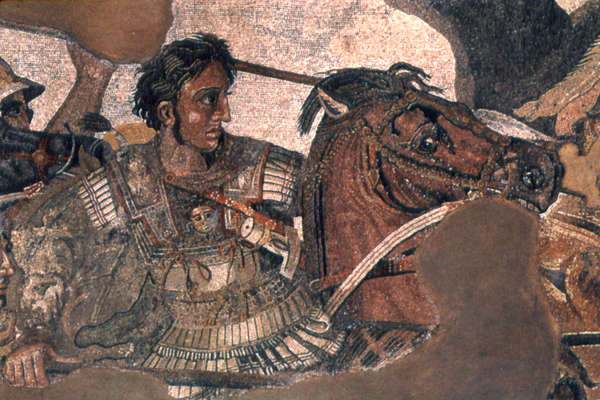
\includegraphics[scale=0.70]{graphics/alexander.jpg}
%     \caption{Detail of the Alexander Mosaic, 1st century \textsc{bc}}
%     \label{fig:alexander}
% \end{figure}
% \begin{figure}[htbp]
%     \centering
%         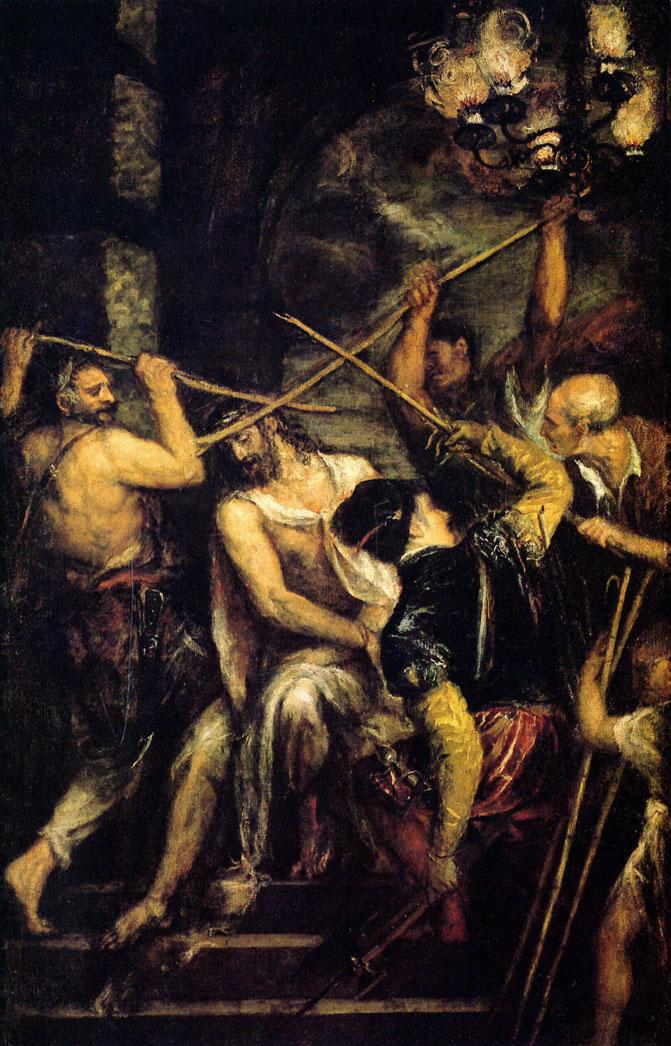
\includegraphics[scale=0.5]{graphics/christ.jpg}
%     \caption{Titian, ``Christ Crowned with Thorns'', 1570}
%     \label{fig:christ}
% \end{figure}

We have seen \citet[29]{Bruno:1977fk}\index{Bruno, Victor J.} claim that in the sophisticated chiaroscuro inaugurated by Zeuxis\index{Zeuxis} ``shading assumed a more dominant role and the nuances of coloring and brushwork became more and more complex, perhaps more `painterly'.'' A sense of this more ``painterly'' style can be seen, according to Bruno, in the figure of Rhadmanthys\index{Rhadmanthys} painted on the facade of the tomb of Lefkadia:\index{tomb of Lefkadia}
\begin{quote}
    A dark is not just an area of darker pink\index{pink} or brown\index{brown} flesh tones; it has blues\index{blue} and greens\index{green} running through it and a complex system of overlapping tones in which every individual stroke is a slightly different color. Color accidents, produced by quick, overlapping brushstrokes, abound throughout the work and are accidents upon which the artist relied. \citep[25]{Bruno:1977fk}
\end{quote}
In the late development of fifth century \textsc{bc} chiaroscuro\index{chiaroscuro}, as light\index{light} and dark\index{dark} come to further dominate the compositional scheme, the relationship between form and color became complicated. Whereas earlier forms of chiaroscuro\index{chiaroscuro} would use one color for shaded parts of a figure, later forms would use a variety of colors, their choice controlled more by relative brightness than hue. The effect of this more complicated scheme may without too much risk of anachronism be described as proto-impressionistic. However, \emph{pace} \citet{Keuls:1975uq}\index{Keuls, Eva}, I do not think that the literary and archeological evidence supports the attribution of nineteenth century ``divisionist''\index{divisionist technique|seealso{pointillism}}\index{pointillism} technique to fifth century \textsc{bc} painters \citep[see][]{Pemberton:1976kx}\index{Pemberton, Elizabeth G.}. However, there need be no ancient predecessor of Suerat\index{Suerat,Georges-Pierre} in fifth century \textsc{bc} painting for there to be a method of color combination that involved not the overlap but the juxtaposition of color.\index{juxtaposition model}

% (see figure~\ref{fig:tomb})
% \begin{figure}[htbp]
%     \centering
%         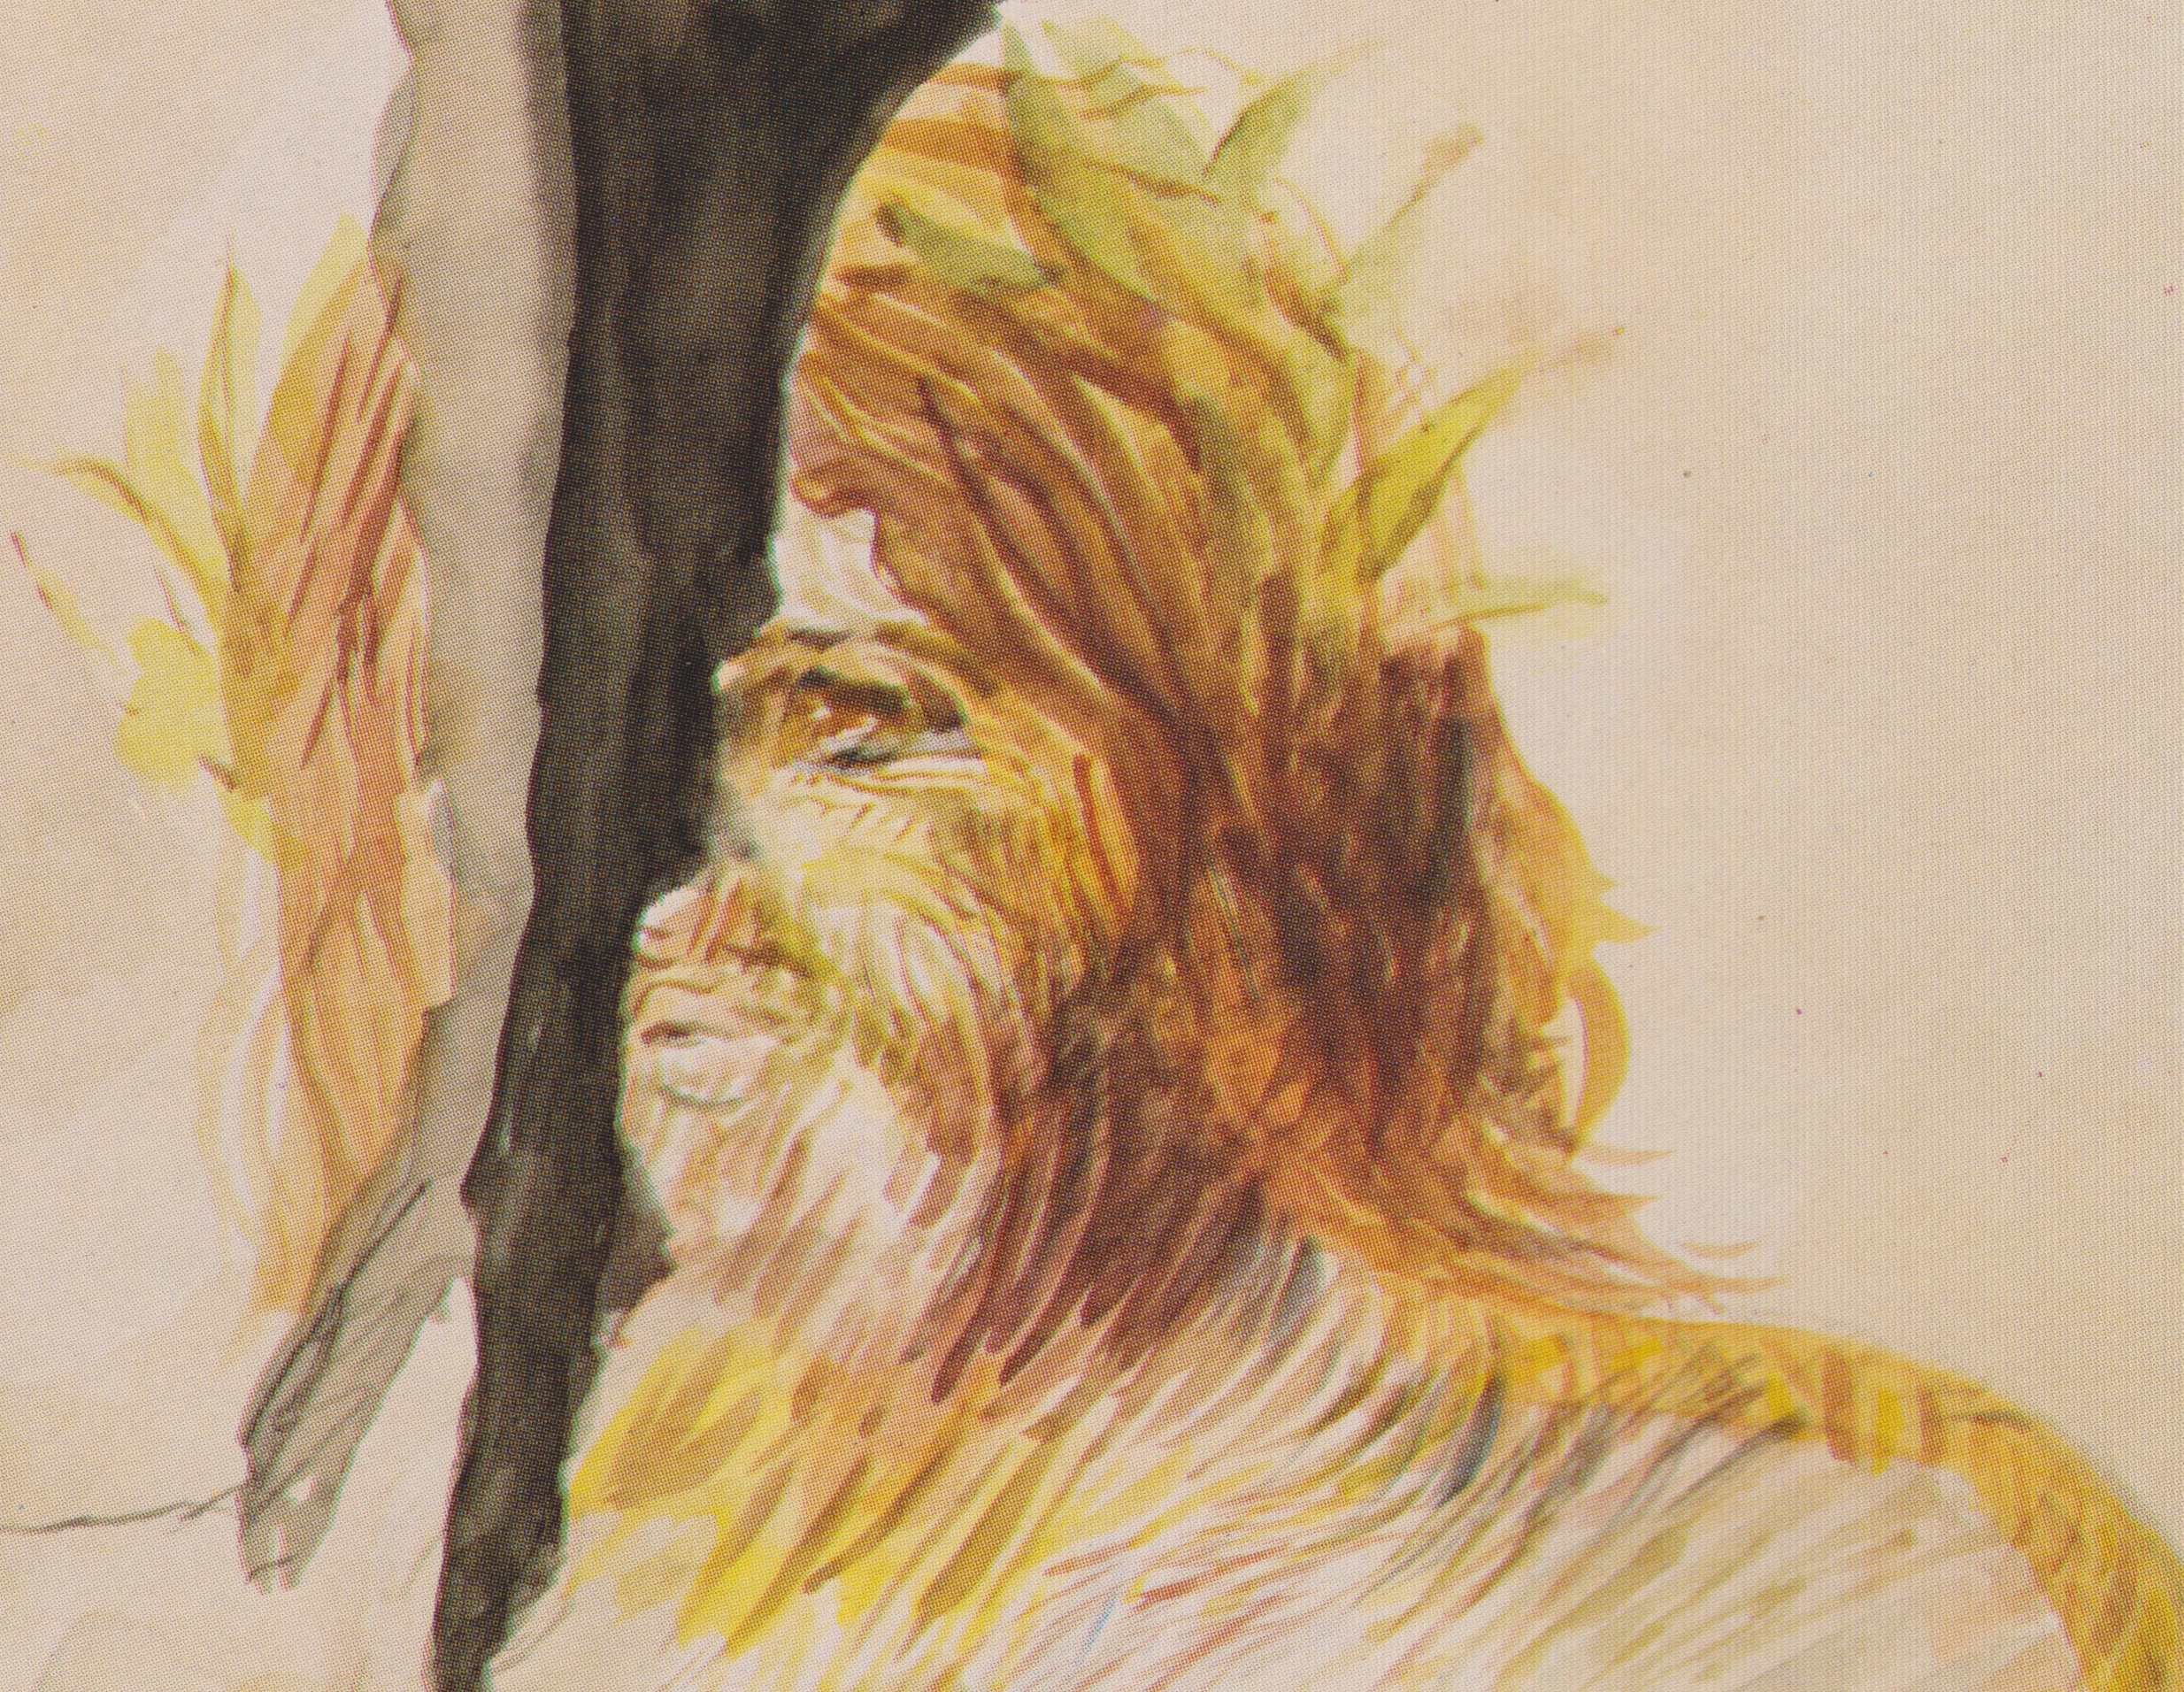
\includegraphics[scale=1]{graphics/tomb.jpeg}
%     \caption{Victor Bruno's watercolor sketch of Rhadamanthys at the tomb of Lefkadia}
%     \label{fig:tomb}
% \end{figure}

We have seen that combination in Empedocles' painting analogy cannot be understood in terms of mixture\index{mixture}. If the sense in which painters combine colors in various proportions to represent the forms of all things is analogous to the sense in which the opposing forces of Love and Strife combine the elements\index{elements} in various proportions, then the metaphysical status of the elements rules out understanding the combination\index{combination} as mixture, since the elements would be indistinguishable in the compound. Fifth century \textsc{bc} painting, however, provides us with two further models. Perhaps the combination could be understood, not in terms of mixture, but in terms of overlap\index{overlap model} or juxtaposition.\index{juxtaposition model} 

In \emph{De Generatione et Corruptione}\index{De Generatione et Corruptione@\emph{De Generatione et Corruptione}}, Aristotle claims that the Empedoclean elements\index{Empedocles!roots} combine by means of juxtaposition and compares the compound to a brick structure:
\begin{quote}
    For how is the manner of their coming-to-be to be conceived by those who maintain a theory like Empedocles? They must conceive it as \emph{composition}---just as a wall comes-to-be out of bricks\index{bricks} and stones\index{stones}: and the `Mixture'\index{mixture}, of which they speak, will be composed out of the `elements'\index{elements}, these being preserved in it unaltered but with their small particles juxtaposed. (Aristotle, \emph{De Generatione et Corruptione}, \textsc{ii} 7 334\( ^{a} \)26--30)
\end{quote}
The Aristotelian interpretation is supported by Galen's\index{Galen} testimony:
\begin{quote}
     For Empedocles says that we, and all the other earthly bodies, are generated from the same elements assumed by Hippocrates, and these elements are not combined with each other, but, as small pieces, stand next to each other, touching. (Galen, \emph{Hippocratis De Naturis Homina Commentaria} \textsc{xv} 49; \textsc{dk} 31\textsc{a}43)\index{Hippocratis De Naturis Homina Commentaria@\emph{Hippocratis De Naturis Homina Commentaria}}
\end{quote}
And Galen\index{Galen} compares the combination of Empedoclean elements to a powder consisting of finely ground metals (\emph{Hippocratis De Naturis Homina Commentaria} 15 32; \textsc{dk} 31\textsc{a}34). Further support for the Aristotelian interpretation comes from an Empedoclean metaphor. Thus he speaks of Love's\index{Empedocles!Love} influence in combining the elements as ``the divine glues of harmony'' (\textsc{dk} 31\textsc{b}96; \citealt[62 245]{Inwood:2001ve}).\index{Empedocles!divine glues of harmony} The metaphor of gluing suggests that the elements ``are not combined with each other, but, as small pieces, stand next to each other, touching''.

If we accept the Aristotelian interpretation, then the combination of the elements should be understood on the model of juxtaposition\index{juxtaposition model}. So, for the analogy to hold,\index{Empedocles!painting analogy} the painter's method of combining colors must itself be understood on the model of juxtaposition, a method arguably associated with the late chiaroscuro inaugurated by Zeuxis\index{Zeuxis} and whose influence can be seen in the tomb of Lefkadia\index{tomb of Lefkadia}. However, Zeuxis' achievement is too late---it arguably post-dates the composition of Empedocles poem(s).  \citet[38--39]{Wright:1981zr}\index{Wright, M.R.}, following \citet[148]{Guthrie:1965ys}\index{Guthrie, W.K.C.}, associates the painter's combining of colors with Apollodorus\index{Apollodorus} and Greek four-color painting\index{four-color palette}. Wright\index{Wright, M.R.} proposes to understand the painter's combining the colors in various proportions with the technique of color combination associated with Greek four-color painting, but that technique works by overlap, not juxtaposition. It is this mismatch that makes me uncertain what positive lessons Empedocles' analogy can provide us about the painter's method of combining colors. It is possible that Aristotle and Galen are right that the Empedoclean combination of elements should be understood on the model of juxtaposition\index{juxtaposition model} \emph{and} that Guthrie and Wright have correctly interpreted the painter's combination of colors in terms of overlaying washes of different colors\index{overlap model}. In which case, the analogy, considered by itself, could serve only to establish the original negative lesson. The combination of the elements is like the combination of the colors in that neither should be understood in terms of blending or mixture. Rather, as it turns out, they work on the models of juxtaposition and overlap, respectively.

How does the combination of elements in various proportions result in the colors of things as they appear in sensory experience? According to A\"{e}tius\index{A\"{e}tius}, four colors---white\index{white}, black\index{black}, red\index{red}, and yellow\index{yellow} (the Greek four-color palette\index{four-color palette})---are assigned to the elements\index{elements}, though A\"{e}tius\index{A\"{e}tius} does not say which color belongs with which element. Partly on this basis some commentators attribute to Empedocles the view that the four elements have four unique colors (\citealt[217]{Cherniss:1935fk}\index{Cherniss, Harold Frederick}, \citealt[152-3]{Siegel:1959fk}\index{Siegel, Rudolph E.}).\index{color!primary} This would be the basis of the desired explanation if the colors of compound bodies were explained in terms of the colors of their constituent elements. Notice that, on such an explanation, white\index{white}, black\index{black}, red\index{red}, and yellow\index{yellow} would be the primary colors---the view that Theophrastus\index{Theophrastus} criticizes Democritus\index{Democritus} for holding (modulo the substitution of yellow\index{yellow} for green\index{green}).  However, the fragments as they come down to us provide no direct support for this interpretation \citep[see][]{Ierodiakonou:2005fk}\index{Ierodiakonou, Katerina}. While Empedocles claims that fire\index{fire} is white\index{white} and water\index{water} is black\index{black}, no specific colors are associated with the other elements\index{elements}. 

I believe that it is more likely that Empedocles is following Parmenides\index{Parmenides} in taking white\index{white} and black\index{black} or light\index{light} and dark\index{dark} as the primary colors\index{color!primary}. As we will see, this interpretation coheres well with Theophrastus'\index{Theophrastus} account of Empedocles' theory of color vision. To illustrate this alternative, let us consider three fragments where Empedocles' associates white with fire and black with water.

Aristotle (\emph{De Anima} \textsc{i} 5 410\( ^{a} \)1)\index{De Anima@\emph{De Anima}} cites the following Empedoclean fragment to illustrate the way in which compound bodies do not merely consist in their constituent elements, but must be combined in a certain proportion:
\begin{verse}
    And pleasant earth in her well-built channels\\
    received two parts of gleaming Nestis\index{Nestis} out of the eight\\
    and four of Hephaistos\index{Hephaistos}; and they become white\index{white} bones\index{bone}\\
    fitted together with the divine glues of harmony\index{Empedocles!divine glues of harmony}.\\
    (Empedocles, \textsc{dk} 31\textsc{b}96; \citealt[62 245]{Inwood:2001ve})
\end{verse}
Nestis\index{Nestis} is a Sicilian water-goddess\index{water}, and Hephaistos\index{Hephaistos} is associated with fire\index{fire}. Thus, according to the fragment, bone\index{bone} is the result of Love's\index{Empedocles!Love} combining four parts fire\index{fire} with two parts earth\index{earth} and two parts water\index{water}. Though some commentators take Nestis\index{Nestis} to refer to water\index{water} and air\index{air}, perhaps under the influence of the general conviction that all four elements are present in every compound body \citep[209 n2]{Wright:1981zr}\index{Wright, M.R.}. On this alternative interpretation, the proportion of elements in bone\index{bone} is four parts fire\index{fire}, two parts earth\index{earth}, one part water\index{water}, and one part air\index{air}. On either interpretation, Empedocles seems to be explaining the whiteness\index{white} of bones\index{bone} in terms of the preponderance of fire\index{fire} in their constituent elements\index{elements}. If we combine this thought with the answer in the style of Gorgias\index{Empedocles!answer in the style of Gorgias} presented in the \emph{Meno}\index{Meno@\emph{Meno}}, then the idea would be that bone\index{bone}, due to the preponderance of fire\index{fire} in its composition, gives off a fiery effluence.\index{Empedocles!effluence!fire} This fiery effluence, due to its distinctive magnitude\index{magnitude}, enters the fire passages\index{Empedocles!passage!fire} in the membrane of the eye and so is made palpable to sight. In this way the whiteness of the bone is manifest in sensory experience.

\citet[301--302]{Palmer:2009qf}\index{Palmer, John} provides an alternative interpretation:
\begin{quote}
	No simple set of ingredients for bone\index{bone} this list implies a procedure whereby the earth is transformed into mud\index{mud} by the addition of water\index{water}, and the resulting compound is hardened by being fired. \citep[302]{Palmer:2009qf}
\end{quote}
Palmer makes an interesting philological case for this alternative interpretation. For our present purposes, the main difficulty with this alternative is that it fails to cohere with the answer in the style of Gorgias\index{Empedocles!answer in the style of Gorgias}. If bone does not contain within itself a preponderance of fire\index{fire}, then it would not give off a fiery effluence. And if bone does not emit fiery effluences\index{Empedocles!effluence!fire}, then it is not white\index{white}, at least according to the answer in the style of Gorgias.

That the color of fire\index{fire} is white\index{white} is further confirmed by a fragment according to which the sun\index{sun} is white\index{white} or bright\index{bright} while rain\index{rain} is black\index{black} or dark\index{dark}:
\begin{verse}
    But come! Gaze on this witness to my previous words,\\
    if anything was in my previous [remarks] left wanting in form:\\
    the sun\index{sun}, bright\index{bright} to look on and hot\index{hot} in every respect,\\
    and the immortals which are drenched in heat\index{hot} and shining light\index{light},\\
    and rain, in all things dark\index{dark} and cold\index{cold};\\
    and there flow from the earth\index{earth} things dense\index{dense} and solid.\\
    (Empedocles, \textsc{dk} 31\textsc{b}21 1--6; \citealt[26 1--6, 229]{Inwood:2001ve})
\end{verse}
Not only then is fire\index{fire}, in the guise of the sun\index{sun}, light\index{light}, but the fragment associates another element with a specific color: The water which composes the rain\index{rain} is dark\index{dark}.

That fire\index{fire} and water\index{water} are the elemental equivalents of light\index{light} and dark\index{dark} is further confirmed by a fragment cited by Plutarch:\index{Plutarch}
\begin{verse}
    And in the depths of the river\index{river} a black\index{black} colour is produced by the shadow\index{shadow},\\
    and in the same way it is observed in cavernous grottoes.\\
    (Empedocles, \textsc{dk} 31\textsc{b}94; \citealt[105 261]{Inwood:2001ve})
\end{verse}
The fragment only explicitly claims that the depths of the river\index{river} is black\index{black}, but Plutarch\index{Plutarch} cites the fragment in answer to the question ``Why does the surface\index{surface} of the water\index{water} look white\index{white} and the depths look black\index{black}?'':
\begin{quote}
    Is it because the depth is the mother of blackness\index{black} inasmuch as it blunts and weakens the sun's\index{sun} rays before they can get to it? But since the surface\index{surface} is immediately affected by the sun, it is reasonable that it receives the gleam of light\index{light}.  (Plutarch, \emph{Historia Naturalis} 39; \citealt[\textsc{ctxt}-87 137--138]{Inwood:2001ve})
\end{quote}
If we accept Plutarch's\index{Plutarch} attribution of this explanation to Empedocles, this supports the elemental equivalence of fire\index{fire} and water\index{water} with light and dark. It also strikingly prefigures the central thought of Aristotle's account of the generation of the hues\index{color!generation of the hues}. Water\index{water} is by nature black\index{black}. However, the color that water appears to have can change depending on whether and to what degree it is illuminated. The surface\index{surface} of water looks white\index{white}, at least in the shifting pattern of reflective highlights. The water near to the surface, where it is not as brightly illuminated, looks blue\index{blue}. And the depths of the river\index{river}, where the sun's\index{sun} rays fail to penetrate, looks black\index{black}. (Compare Aristotle's claim that the sea\index{sea} is an imperfectly transparent\index{transparency!degrees of} medium\index{medium} that appears differently near or far \emph{De Sensu} \textsc{iii} 439\( ^{b} \)1--3 and his claim that water\index{water} looks darker the deeper and less transparent it is \emph{De Generatione Animalium} \textsc{v} 779\( ^{b} \)27--33, 780\( ^{b} \)8.)\index{De Generatione Animalium@\emph{De Generatione Animalium}} The different colors---white\index{white}, blue\index{blue}, and black\index{black}---are due to different different proportions\index{proportion} of fire\index{fire} and water\index{water}. In the shifting pattern of reflective highlights\index{highlight}, there is a preponderance of fire\index{fire} and this results in a brilliant appearance\index{bright}; whereas, in the depth of the river\index{river}, there is a preponderance of water\index{water} (and perhaps no fire at all) and this results in a dark\index{dark} appearance. In the shallows of the river\index{river}, due to a more equitable combination of fire and water, a blue appearance is manifest.

Accepting Plutarch's\index{Plutarch} attribution, and generalizing it, thus results in the following picture: White\index{white} and black,\index{black} like hot\index{hot} and cold\index{cold}, are sensible qualities\index{sensible qualities} paired with their contrary\index{contraries}. And like hot and cold, white and black are the endpoints of an ordered range of sensible qualities\index{sensible qualities}. That the range is ordered as a continuum\index{continuum} is a further claim. Aristotle, for one, denies it (\emph{De Sensu} \textsc{vi})\index{De Sensu@\emph{De Sensu}}. Blue\index{blue} is a sensible quality\index{sensible qualities} located somewhere between the extremes of white\index{white} and black\index{black} as is every other color\index{color}. Blue\index{blue} is perhaps more dark than light just as yellow\index{yellow} is more light than dark. In this regard, Empedocles' theory shares a feature with the Homeric color scheme\index{Homer!color scheme} of which \citet[458]{Gladstone:1858fk}\index{Gladstone, W.E.} complained, namely, ``the decided tendency to treat other colours as simply intermediate modes between these two extremes'', that is, ``the crude and elemental forms of colour, black and white''. Moreover, the relevant proportion\index{proportion} of light\index{light} and dark\index{dark} is determined by the substance's\index{substance} elemental\index{elements} composition. The proportion of light and dark that results in the blue\index{blue} of the river's\index{river} shallows is determined by the proportion\index{proportion} of fire\index{fire} and water\index{water} in its composition. Specifically, the fiery emission of the sun\index{sun} penetrates to some degree the shallows of the river\index{river}, and it is the resulting proportion of fire\index{fire} and water\index{water} that determines the proportion of light and dark of which the shallows partake. 

This constitutes a means for addressing one of Theophrastus'\index{Theophrastus} complaints. Theo\-phrastus concedes that on Empedocles' account, the perception of white\index{white} and black\index{black} is relatively straightforward. In the membrane\index{Empedocles!perception!membrane} of the eye\index{eye} there are alternating passages of fire\index{Empedocles!passage!fire} and water\index{Empedocles!passage!water}. White effluences\index{Empedocles!effluence!chromatic} emitted from distal objects are assimilated by fire passages, black effluences are assimilated by water passages, and so each is made palpable to the organ of sight. But how, on this model, is the perception of the chromatic hues\index{hue} to be explained? Theophrastus\index{Theophrastus} complains that Empedocles owes us an explanation but has failed to provide one:
\begin{quote}
	Now since, for him, the eye is composed of fire and of its opposite, it might well recognize white\index{white} and black\index{black} by means of what is like them; but how could it become conscious of gray\index{gray} and the other compound colours? For he assigns <their perception> neither to the minute passages of fire\index{Empedocles!passage!fire} nor to those of water\index{Empedocles!passage!water} nor to others composed of both these elements together. Yet we see the compound colours no whit less than we do the simple. (Theophrastus, \emph{De Sensibus} \textsc{xvii}; \citealt[81]{Stratton:1917vn})
\end{quote}

The elemental composition of a distal object, specifically, its proportion\index{proportion} of fire\index{fire} and water\index{water}, determines the amount of fiery and watery effluences\index{Empedocles!effluence!fire}\index{Empedocles!effluence!water} it emits. Fiery effluences are white\index{white}. Watery effluences are black\index{black}. A purely white object, such as a noon sun\index{sun} on a clear summer's day\index{day}, emits only fiery effluences. A purely black object, such as the river's\index{river} depths, emits only watery effluences. \index{Empedocles!effluence!chromatic}Objects with chromatic hues emit a proportion of fiery\index{Empedocles!effluence!fire} and watery\index{Empedocles!effluence!water} effluences corresponding the proportion of fire and water in its elemental composition. Thus the river's\index{river} shallows emits a proportion of fiery and watery effluences (the fiery effluences being the sun's contribution in penetrating the river). These fiery and watery effluences are assimilated, respectively, by the fire and water passages in the membrane of the eye. And, arguably at least, it is the proportion of fire and water assimilated that gives rise to the perception of blue. 

Theophrastus\index{Theophrastus} complained that Empedocles assigns the perception of compound colors ``neither to the minute passages of fire nor to those of water nor to others composed of both these elements together.''\index{Empedocles!passage!fire}\index{Empedocles!passage!water} It is true that the perception of blue\index{blue} is not assigned to the fire passages in the eye's membrane\index{Empedocles!perception!membrane}, nor to its water passages. Whether it is explained in terms of ``others composed of both these elements'' depends on what exactly Theophrastus\index{Theophrastus} means here. Perhaps he means that just as there are fire and water passages in the membrane of the eye, there are other passages, as well, that are commensurate with effluences compounded out of fire and water. So understood, Theophrastus\index{Theophrastus} is right not to attribute this doctrine to Empedocles. However, there is another alternative. The passages in the membrane\index{Empedocles!perception!membrane} of the eye\index{eye} consist solely of alternating fire and water passages\index{Empedocles!passage!fire}\index{Empedocles!passage!water}. There are no other kinds of passages to be found. A chromatic hue\index{hue} is just the proportion\index{proportion} of fiery and watery effluence\index{Empedocles!effluence!fire}\index{Empedocles!effluence!water} emitted by a distal object, and its perception is the resulting proportion of assimilated fire and water being made palpable to the organ of sight.\index{color!generation of the hues} Like all things on earth and in heaven, at least in a certain stage of the cosmic cycle, the chromatic hues and their perception are the result of Aphrodite's\index{Aphrodite} Love\index{Empedocles!Love}, the principle of harmony\index{harmony}, counteracting the operation of Strife.\index{Empedocles!Strife}
\index{Empedocles|)}

% section empedocles (end)

% chapter light_and_dark (end)